\documentclass[a4paper]{article}
\usepackage[utf8]{inputenc}
\usepackage[natbib,sorting=none]{biblatex}
\usepackage{graphicx}
\usepackage{acronym}
\usepackage{indentfirst}
\usepackage[htt]{hyphenat}
\usepackage{fancyhdr}
\usepackage{enumitem}
\usepackage{listings}
\usepackage{xcolor}
\usepackage{pifont}

\addbibresource{references.bib}
\newcommand{\comment}[1]{\textbf{[Comment: #1]}}

\begin{document}
\setlist[enumerate]{label=\alph*),leftmargin=0.4cm, topsep=0cm}
\setlist[itemize]{leftmargin=0.4cm, topsep=0cm}
\begin{figure}[!h]
	\centering
	
\includegraphics[width=80mm]{images/poli-logo.png}
\end{figure}
\hfill
\begin{center}
    \fontsize{18px}{6mm}\selectfont \textsc{\textbf{Software Engineering II project}}
\end{center}
\begin{center}
    \fontsize{12px}{4mm}\selectfont \textsc{Academic Year: 2018/2019}
\end{center}
\hfill
\hfill
\begin{figure}[!h]
	\centering
	
\includegraphics[width=120mm]{images/trackme-logo.png}
\end{figure}
\hfill
\hfill
\begin{center}
    \fontsize{22px}{8mm}\selectfont \textsc{\textbf{Requirement Analysis and\\ Specification Document}}
\end{center}
\begin{center}
    \fontsize{14px}{4mm}\selectfont \textsc{{Draft Version 0.1 - 11/10/2018}}
\end{center}
\hfill
\hfill
\begin{center}
\fontsize{14px}{4mm}\selectfont \textsc{\textit{Davide Rutigliano -  903616}}
\end{center}

\begin{center}
\fontsize{14px}{4mm}\selectfont \textsc{\textit{Claudio Ferrante - 903417\\}}
\end{center}

\begin{center}
\fontsize{14px}{4mm}\selectfont \textsc{\textit{Davide Matta - 903616}}
\end{center}
\pagenumbering{roman}
\tableofcontents
\rfoot{
\includegraphics[width=30mm]{Images/trackme-logo-mini.png}}

%%%%%%%%%%%%%%%%%%%%%%%%%%%%%%%%%%%%%%%%%%%%%%%%%%%%%%%%%%%%%%%%%%%%%%
\newpage
\pagestyle{fancy}
\pagenumbering{arabic}

\section{Introduction}

\subsection{Purpose}
    The Purpose of this Design Document is to provide, in a more specific and technical way with regard to the RASD, all the details of \textit{TrackMe} system.
    
    In particular, this document is addressed to  developers team. Through this paper they can better understand and identify: the main components and their interfaces and their behaviours, the high level architecture and its interaction with architectural components; style and design patterns that shall be used in deployment of the application.
    
    Furthermore this document provides also an \textit{Implementation \& Test} plan.
 
    \subsection{Scope}
    \textit{TrackMe} system has been project in such a way that it is a service available on web and mobile application. The subjects the should use this service can belong to two different categories:
    \newline
    \begin{itemize}
    
    \item{Individuals}
    
    \item{Third-Party}
    \newline
    \end{itemize}
    
   
   \textit{TrackMe} give allows Third-Party to access Individual's health data exploiting the functionalities of \textit{Data4help} section of \textit{TrackMe}. The Third-Parties can make Individual, or group request. the Individuals  can accept or not Third-parties' requests. The application may also allow individual users to connect external  devices such as smart-watches or similar, to perform a more detailed data acquisition and monitoring. 
   \newline
   
   
   In addition, the third-party may also provide a personalized and non intrusive SOS service for elderly people who requested it.
   The system permits to enable the \textit{Automated-SOS} service that guarantees that the GPS position of an user, who has enabled \textit{Automated SOS}, can be send to the nearest ambulance available, when user's health parameters overcome some critical thresholds. This procedure takes place thanks to an ambulance dispatcher, which is connected to the Third-Party (which has enabled automated-SOS too), that has been selected by that individual to provide this service
   \newline
   
   
   Moreover,  through  the \textit{Track4Run} service, \textit{TrackMe} allows \textit{Organizers} (that are individuals)  to  \textit{create}  a  new  run:  a  competition  in  which other individuals can either participate as \textit{athletes} or watch as \textit{spectators}.  Additionally, this feature guarantees other services for keeping track of athletes progresses during the run, providing an interactive map of the run, with runners position on it.

\subsection{Definition, Acronyms and  Abbreviations}
           
            \subsubsection{Definition of Terms}
            This document uses several terms that might be more loosely used elsewhere. These terms are defined here as they will be used later on in this document.
                \begin{description}
                    \item[\textbf{Subscribed User}] an individual for which one or more third party have done a request accepted by the individual itself
                    
                    \item[\textbf{External Device}] an external device such as a smart-watch or similar devices
                    
                    \item[\textbf{Run}] a competition organized and managed by an \textit{Organizer} to which \textit{Athletes} and \textit{Spectators} can enroll as participant or watchers
                    
                    \item[\textbf{Run Started}] a competition with at least two \textit{Athletes} enrolled that the \textit{Organizer} has started
                    
                    \item[\textbf{Run Not-Started}] a competition with any number of \textit{Athletes} enrolled
                    
                    \item[\textbf{Map}] The map of the predefined track of the run with athletes' positions
                    
                    \item[Accident] An event triggered when the monitored user's parameter overcome certain thresholds
                    
                    \item[\textbf{TrackMe}] the \textit{"system to be"}
                    
                    \item[\textbf{Data4Help}] a data monitoring service provided by \textit{TrackMe}
                    
                    \item[\textbf{Automated-SOS}] an SOS service built on top of \textit{Data4Help}
                    
                    \item[\textbf{Track4Run}] run management service offered by \textit{TrackMe} application
                    
                    \item[\textbf{Credential}] as used in this document, is a combination of both username and password used by an \textit{User} to authenticate him/herself during the Log-in phase
                    
                    \item[\textbf{Personal Data}] users' data of different kind either for Individuals (name, surname, age, etc.) or for Third-Parties such as Organization name, number of employees or VAT number
                \end{description}
                
            
            \subsubsection{Acronyms}
            \begin{acronym}
                \acro{DD}{Design Document}
                \acro{UML}{Unified Modelling Language}
                \acro{REST}{REpresentational State Transfer}
                \acro{API}{Application Programming Interface}
            \end{acronym}
            
            \subsubsection{Abbreviations}
            
\subsection{Reference Documents}

\printbibliography[heading=none]

%%%%%%%%%%%%%%%%%%%%%%%%%%%%%%%%%%%%%%%%%%%%%%%

\newpage

\subsection{Document Structure}
%% questa parte è presa pari pari dal DD su beep


\begin{itemize}
    \item \textbf{Introduction}: this section introduces the design document. It contains
a justification of his utility and indications on which parts are covered in
this document that are not covered by RASD.

\item \textbf{Architecture Design}: this section is divided into different parts:
\begin{enumerate}
    \item Overview : this sections explains the division in tiers of our application
    
    \item High level components and their interaction : this sections gives
a global view of the components of the application and how they
communicate

    \item Component view : this sections gives a more detailed view of the
components of the applications

    \item Deploying view : this section shows the components that must be
deployed to have the application running correctly.

    \item Runtime view : sequence diagrams are represented in this section to
show the course of the different tasks of our applicatio

    \item Component interfaces : the interfaces between the components are
presented in this section

    \item Selected architectural styles and patterns : this section explain the
architectural choices taken during the creation of the application

    \item Other design decisions
    
\end{enumerate}


\item \textbf{Algorithms Design}: this section describes the most critical parts via
some algorithms. Pseudo code is used in order to hide unnecessary implementation
details in order to focus on the most important parts.


\item \textbf{User Interface Design}: this section presents mockups and user experience
explained via UX and BCE diagrams


\item \textbf{Requirements Traceability}: this section aims to explain how the decisions
taken in the RASD are linked to design elements
\end{itemize}

\newpage

\section{Architectural Design}

%%%%%%%%%%%%%%%%%%%%%%%%%%%%%%%%%%%%%%%%5

%questa sezione richiede uno studio aprofondito, ne do un abbozzo e poi ne discutiamo insieme, serve anche un diagramma-schema

On the client side it is possible a communication with the server through a module that can send API calls to the server. This can be done both with the mobile applications and with browser on web applications.
%%dovremmo forse utilizzare solo una mobile app ?
The data server is separeted by the Application one.



%%%%%%%%%%%%%%%%%%%%%%%%%%%%%%%%%%%%%%%%%

\subsection{Overview: High-level components and their interaction}

The components that charcterise our system are:

\begin{itemize}
    \item \textbf{Application Server}: This tier comprises all the logic of the application system. This includes the main algorithms and the logic to intercat with external systems
    
    \item \textbf{Mobile Application}: The presentation layer.
it allows to communicate with the application server and the only logic used is the presentation one .

   \item \textbf{Database} The data layer of the system; it enclose all the structures for data management. The only logic present is the Database Management system, DBMS. It ensures that the ACID properties are granted.
\end{itemize}

%%completare questa sezione, magari con uno schema con relativa descrizione, basandosi sulla versione precedente

\newpage

\subsection{Component view}


 
    
    \begin{figure}[!htpb]
        \centering
        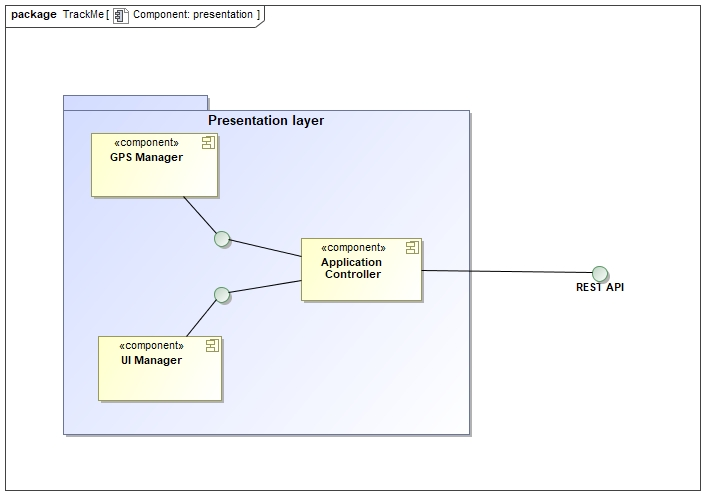
\includegraphics[width=\textwidth]{DD/images/CP.jpg}
        \caption{Component diagram: presentation layer}
    \end{figure}
    \newpage





\subsection{Deployment view}

\subsection{Runtime view}

\subsection{Component interfaces}

\subsection{Selected architectural styles and patterns}

\subsection{Other design decisions}

\section{User Interface Design}

        \begin{figure}[!htpb]
    	\centering
    	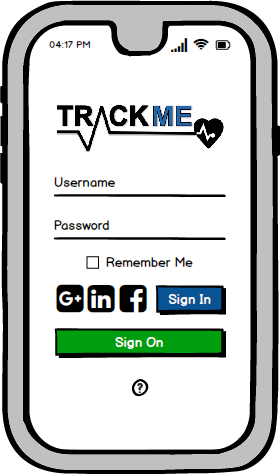
\includegraphics[height=50mm]{images/mockups/Login_Registration.png}
    	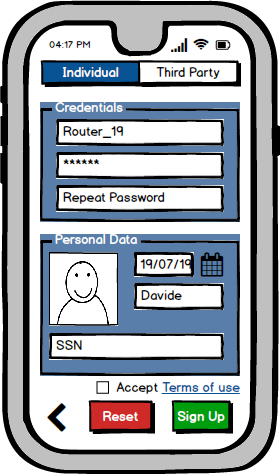
\includegraphics[height=50mm]{images/mockups/RegistrationForm.png}
    	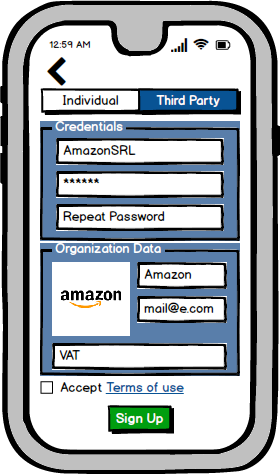
\includegraphics[height=50mm]{images/mockups/ThirdPartyRegistration.png}
        \end{figure}
        
        \begin{figure}[!htpb]
    	\centering
    	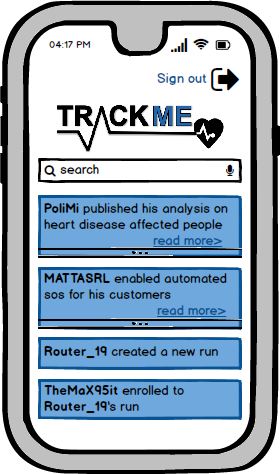
\includegraphics[height=50mm]{images/mockups/HomePage.png}
    	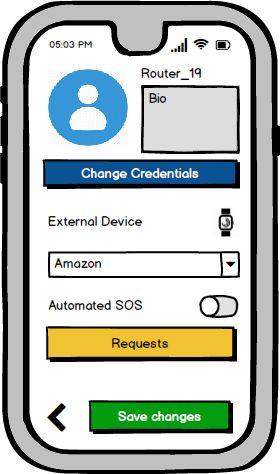
\includegraphics[height=50mm]{images/mockups/IndividualProfile.png}
    	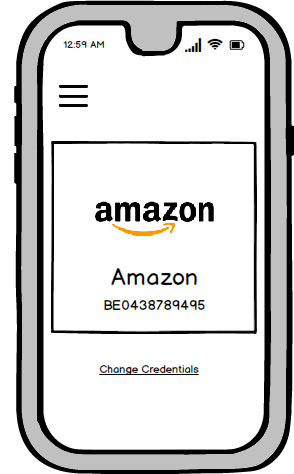
\includegraphics[height=50mm]{images/mockups/ThirdPartyProfile.png}
        \end{figure}
        
        \begin{figure}[!htpb]
    	\centering
    	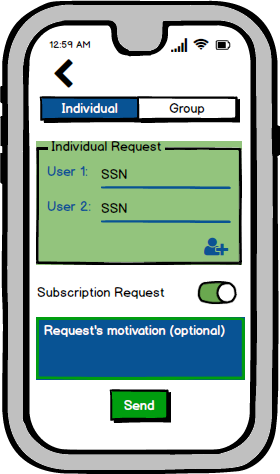
\includegraphics[height=50mm]{images/mockups/Requests.png}
    	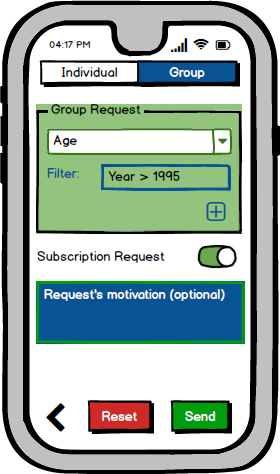
\includegraphics[height=50mm]{images/mockups/GroupRequest.png}
    	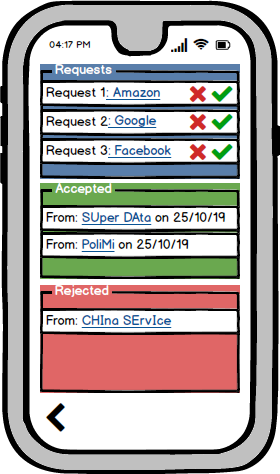
\includegraphics[height=50mm]{images/mockups/ManageRequests.png}
    	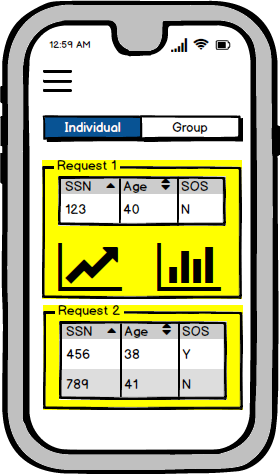
\includegraphics[height=50mm]{images/mockups/ViewData.png}
    	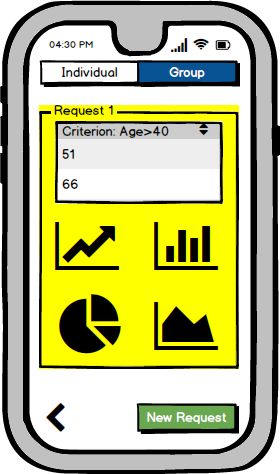
\includegraphics[height=50mm]{images/mockups/ViewData2.png}
        \end{figure}
        
        \begin{figure}[!htpb]
    	\centering
    	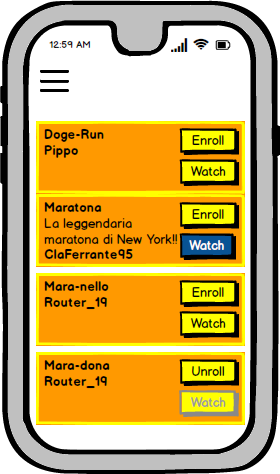
\includegraphics[height=50mm]{images/mockups/RunManager.png}
    	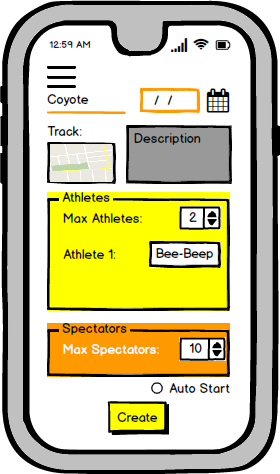
\includegraphics[height=50mm]{images/mockups/RunCreate.png}
    	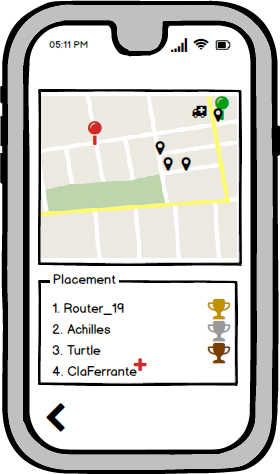
\includegraphics[height=50mm]{images/mockups/ShowMap.png}
    	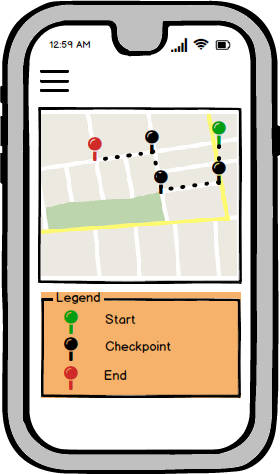
\includegraphics[height=50mm]{images/mockups/DefineTrack.png}
        \end{figure}
        
\section{Requirements Traceability}

\section{Implementation, Integration and Test Plan}

\section{Effort Spent}

\end{document}